\documentclass{article}
% generated by Madoko, version 1.1.3
%mdk-data-line={1}


\usepackage[heading-base={2},section-num={False},bib-label={hide},fontspec={True}]{madoko2}
\usepackage[UTF8]{ctex}


\begin{document}



%mdk-data-line={3}
\section{\mdline{3}1.\hspace*{0.5em}\mdline{3}Elasticsearch与solr的对比}\label{sec-elasticsearchsolr}%mdk%mdk

%mdk-data-line={5}
\subsection{\mdline{5}1.1.\hspace*{0.5em}\mdline{5}官网资料}\label{section}%mdk%mdk

%mdk-data-line={6}
\begin{itemize}[noitemsep,topsep=\mdcompacttopsep]%mdk

%mdk-data-line={6}
\item\mdline{6}es: https://www.elastic.co/guide/en/elasticsearch/reference/current/index.html(从tutorial到详细的api使用)%mdk

%mdk-data-line={7}
\item\mdline{7}solr: http://mirror.bit.edu.cn/apache/lucene/solr/ref-guide/apache-solr-ref-guide-6.6.pdf (900多页的文档,十分详尽)%mdk
%mdk
\end{itemize}%mdk

%mdk-data-line={9}
\subsection{\mdline{9}1.2.\hspace*{0.5em}\mdline{9}分布式架构\mdline{9}\&\mdline{9}分布式部署}\label{section}%mdk%mdk

%mdk-data-line={10}
\subsubsection{\mdline{10}1.2.1.\hspace*{0.5em}\mdline{10}分布式架构}\label{section}%mdk%mdk

%mdk-data-line={11}
\begin{itemize}%mdk

%mdk-data-line={11}
\item{}
%mdk-data-line={11}
\mdline{11}es: 基于自身的node特性,不需要接入其他服务构建集群,自身有一个“自动发现”的特性,可以通过一个端口检测其他节点并于其他节点通信。相关配置如下:    \mdline{11}\mdbr
\mdline{12}discovery.zen.ping.unicast.hosts(设置集群中master节点的初始列表,可以通过这些节点来自动发现新加入集群的节点)    \mdline{12}\mdbr
\mdline{13}discovery.zen.minimum\mdline{13}\_\mdline{13}master\mdline{13}\_\mdline{13}nodes(设置这个参数来保证集群中的节点可以知道其它N个有master资格的节点,若少于这个数,集群其他节点也不会工作)    \mdline{13}\mdbr
\mdline{14}支持主节点自动选举。管理web界面(Kibana的x-pack插件或head插件)%mdk%mdk

%mdk-data-line={16}
\item{}
%mdk-data-line={16}
\mdline{16}solr:基于zookeeper建立集群,便于管理。通过zk自动发现集群你得节点。支持主节点自动选举(zk特性)。
管理web界面(solr自带)    \mdline{17} \mdline{17}%mdk%mdk
%mdk
\end{itemize}%mdk

%mdk-data-line={19}
\subsubsection{\mdline{19}1.2.2.\hspace*{0.5em}\mdline{19}数据分片与备份}\label{section}%mdk%mdk

%mdk-data-line={20}
\begin{itemize}[noitemsep,topsep=\mdcompacttopsep]%mdk

%mdk-data-line={20}
\item\mdline{20}es: 可以指定特定数据项的数据分片数以及数据备份数。在数据导入过程中配置。相关配置项如下:    \mdline{20} \mdline{20}%mdk
%mdk
\end{itemize}%mdk

%mdk-data-line={22}
\begin{mdcenter}%mdk

%mdk-data-line={23}
\noindent\mdline{23}\textquotedblleft{}number\_of\_shards\textquotedblright{}\mdline{23} : 3,     \mdline{23}\mdbr
\mdline{24}\textquotedblleft{}number\_of\_replicas\textquotedblright{}\mdline{24} : 1%mdk
%mdk
\end{mdcenter}%mdk

%mdk-data-line={27}
\begin{mdcenter}%mdk

%mdk-data-line={28}
\noindent\mdline{28}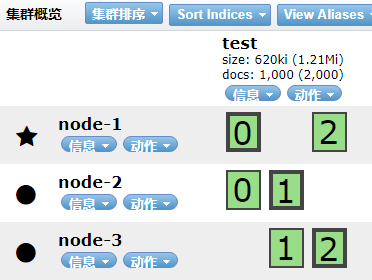
\includegraphics[keepaspectratio=true,width=\dimmin{}{\dimwidth{0.90}}]{images/test}{}\mdline{28}%mdk
%mdk
\end{mdcenter}%mdk

%mdk-data-line={34}
\noindent\mdline{34}如上图所示,表示数据进行了三分片两备份。%mdk

%mdk-data-line={36}
\begin{itemize}[noitemsep,topsep=\mdcompacttopsep]%mdk

%mdk-data-line={36}
\item\mdline{36}solr: 与es相同,同样可指定。相关配置项如下:    \mdline{36} \mdline{36} 

%mdk-data-line={37}
\begin{mdcenter}%mdk

%mdk-data-line={38}
\noindent\mdline{38}-shards 2\mdline{38} \mdline{38}-replicationFactor 2%mdk
%mdk
\end{mdcenter}%mdk%mdk
%mdk
\end{itemize}%mdk

%mdk-data-line={41}
\subsubsection{\mdline{41}1.2.3.\hspace*{0.5em}\mdline{41}集群监控}\label{section}%mdk%mdk

%mdk-data-line={42}
\begin{itemize}[noitemsep,topsep=\mdcompacttopsep]%mdk

%mdk-data-line={42}
\item\mdline{42}es: 通过Http Restful Api检测集群健康状况%mdk

%mdk-data-line={43}
\item\mdline{43}solr: 通过JMX可与Prometheus结合监控状态%mdk
%mdk
\end{itemize}%mdk

%mdk-data-line={45}
\subsection{\mdline{45}1.3.\hspace*{0.5em}\mdline{45}数据导入}\label{section}%mdk%mdk

%mdk-data-line={46}
\subsubsection{\mdline{46}1.3.1.\hspace*{0.5em}\mdline{46}数据格式}\label{section}%mdk%mdk

%mdk-data-line={47}
\begin{itemize}[noitemsep,topsep=\mdcompacttopsep]%mdk

%mdk-data-line={47}
\item\mdline{47}es: 仅支持json的导入,但是由第三方很多的序列化方法可供使用。%mdk

%mdk-data-line={48}
\item\mdline{48}solr: 支持多种格式,json、csv、xml%mdk
%mdk
\end{itemize}%mdk

%mdk-data-line={50}
\subsubsection{\mdline{50}1.3.2.\hspace*{0.5em}\mdline{50}数据从mysql导入,同步}\label{sec-mysql}%mdk%mdk

%mdk-data-line={51}
\begin{itemize}%mdk

%mdk-data-line={51}
\item{}
%mdk-data-line={51}
\mdline{51}es:%mdk

%mdk-data-line={53}
\mdline{53}1、通过elasticsearch-jdbc插件可导入。(已测试可导入)。    \mdline{53}\mdbr
\mdline{54}2、同样的,可通过这个插件进行\mdline{54}\href{https://www.elastic.co/guide/en/logstash/current/plugins-inputs-jdbc.html}{数据同步}\mdline{54}(近实时)。原理:通过logstash监听数据库的某个表。可自定义检查时间间隔以及sql来定制需要同步的字段,实现数据库的操作(insert、update等)自动同步至es。(未测试)    \mdline{54}\mdbr
\mdline{55}3、支持kettle导入%mdk%mdk

%mdk-data-line={57}
\item{}
%mdk-data-line={57}
\mdline{57}solr: 目前找到方法为定时与手动方法,可增量、全量同步数据。配置db-data-config.xml,可定制导入字段,通过web管理界面或代码(solrj)实现导入。%mdk%mdk
%mdk
\end{itemize}%mdk

%mdk-data-line={59}
\subsection{\mdline{59}1.4.\hspace*{0.5em}\mdline{59}搜索语法、包装成本、Java支持\mdline{59}\&\mdline{59}中文分词支持}\label{sec-java}%mdk%mdk

%mdk-data-line={60}
\noindent\mdline{60}\mdref{section}{注:原生的es和solr对中文的分词可以说是跟没有一样,只是简单的把字分开而已,es可以设置单字或双字模式。}\mdline{60}      \mdline{60} \mdline{60}%mdk

%mdk-data-line={62}
\begin{itemize}%mdk

%mdk-data-line={62}
\item{}
%mdk-data-line={62}
\mdline{62}es:    \mdline{62} \mdline{62}%mdk

%mdk-data-line={64}
\mdline{64}1、Http Restful Api    \mdline{64}\mdbr
\mdline{65}2、Client: 对Java支持很好,通过连接串拿到es\mdline{65}\_\mdline{65}client。(官方多语言支持,Java、Python、javascript\mdline{65}\dots{}\mdline{65})    \mdline{65}\mdbr
\mdline{66}3、如果不使用Client方法,专门使用Http Restful Api
es提供了如下两种请求格式:    \mdline{67}\mdbr
\mdline{68}REST request URI, 例如:    \mdline{68} \mdline{68}%mdk
\begin{mdpre}%mdk
\noindent GET~{\mdcolor{maroon}/}{\mdcolor{maroon}b}{\mdcolor{maroon}a}{\mdcolor{maroon}n}{\mdcolor{maroon}k}{\mdcolor{maroon}/}\_search?q=*\&sort=account\_number:asc\&pretty%mdk
\end{mdpre}
%mdk-data-line={72}
\mdline{72}REST request body, 例如:%mdk
\begin{mdpre}%mdk
\noindent GET~{\mdcolor{maroon}/}{\mdcolor{maroon}b}{\mdcolor{maroon}a}{\mdcolor{maroon}n}{\mdcolor{maroon}k}{\mdcolor{maroon}/}\_search\\
\{\\
{\mdcolor{maroon}"}{\mdcolor{maroon}query}{\mdcolor{maroon}"}:~\{~{\mdcolor{maroon}"}{\mdcolor{maroon}match\_all}{\mdcolor{maroon}"}:~\{\}~\},\\
{\mdcolor{maroon}"}{\mdcolor{maroon}sort}{\mdcolor{maroon}"}:~{}[\\
~~\{~{\mdcolor{maroon}"}{\mdcolor{maroon}account\_number}{\mdcolor{maroon}"}:~{\mdcolor{maroon}"}{\mdcolor{maroon}asc}{\mdcolor{maroon}"}~\}\\
]\\
\}%mdk
\end{mdpre}
%mdk-data-line={82}
\mdline{82}4、es有一套成熟的DSL,可以做十分复杂的过滤、聚合、查找、分页的query。    \mdline{82}\mdbr
\mdline{83}5、中文分词:elasticsearch-analysis-ik、elasticsearch-hanlp等第三方插件,并且插件很多,可对比效果使用    \mdline{83}\mdbr
\mdline{84}6、在title里面添加zh和en两个fields,这样对中文,英文都分别使用分词器,title.zh使用ik分词,title.en使用英文分词,搜索可同时覆盖。%mdk%mdk

%mdk-data-line={86}
\item{}
%mdk-data-line={86}
\mdline{86}solr:%mdk

%mdk-data-line={88}
\mdline{88}1、Http Restful Api    \mdline{88}\mdbr
\mdline{89}2、Client: solrj(maven:solr-solrj)(官方只支持Java)    \mdline{89}\mdbr
\mdline{90}3、conf下的managed-schema.xml配置文件中配置中文分词:IK Analyzer/mmseg4j   (可配词库)    \mdline{90}\mdbr
\mdline{91}4、有全文本搜索过滤主要还是查找功能。%mdk%mdk
%mdk
\end{itemize}%mdk

%mdk-data-line={96}
%mdk-data-line={97}
\noindent\mdline{97}Enjoy! By Hanbing.    \mdline{97}\mdbr
\mdline{98}Using madoko.%mdk%mdk%mdk


\end{document}
